\section{Документация к программе}

Документация к программе --- это один из самых важных аспектов в разработке
программного обеспечения. В рамках курсовой работы на тему ``Разработка
распределенной асинхронной системы обработки real-time финансовых данных'' было
уделено большое внимание документированию API приложения. Для этого было
использовано OpenAPI.

OpenAPI --- это язык описания RESTful API, который позволяет разработчикам
создавать и документировать API для своих приложений. Он позволяет определить
все доступные ресурсы, методы, параметры и схемы данных, которые используются в
приложении. OpenAPI является полезным инструментом для разработчиков, поскольку
он помогает им легко создавать и поддерживать API, а также упрощает процесс
интеграции с другими приложениями.

Для документирования API приложения было использовано Swagger UI ---
инструмент, который позволяет визуально отображать и тестировать API. На рисунке \ref{swager}
вы можете увидеть пример того, как выглядит документация нашего API в Swagger UI.
Здесь можно увидеть все доступные ресурсы, методы и параметры, а также выполнить
тестирование каждого метода.

\begin{figure}[h]
    \centering
    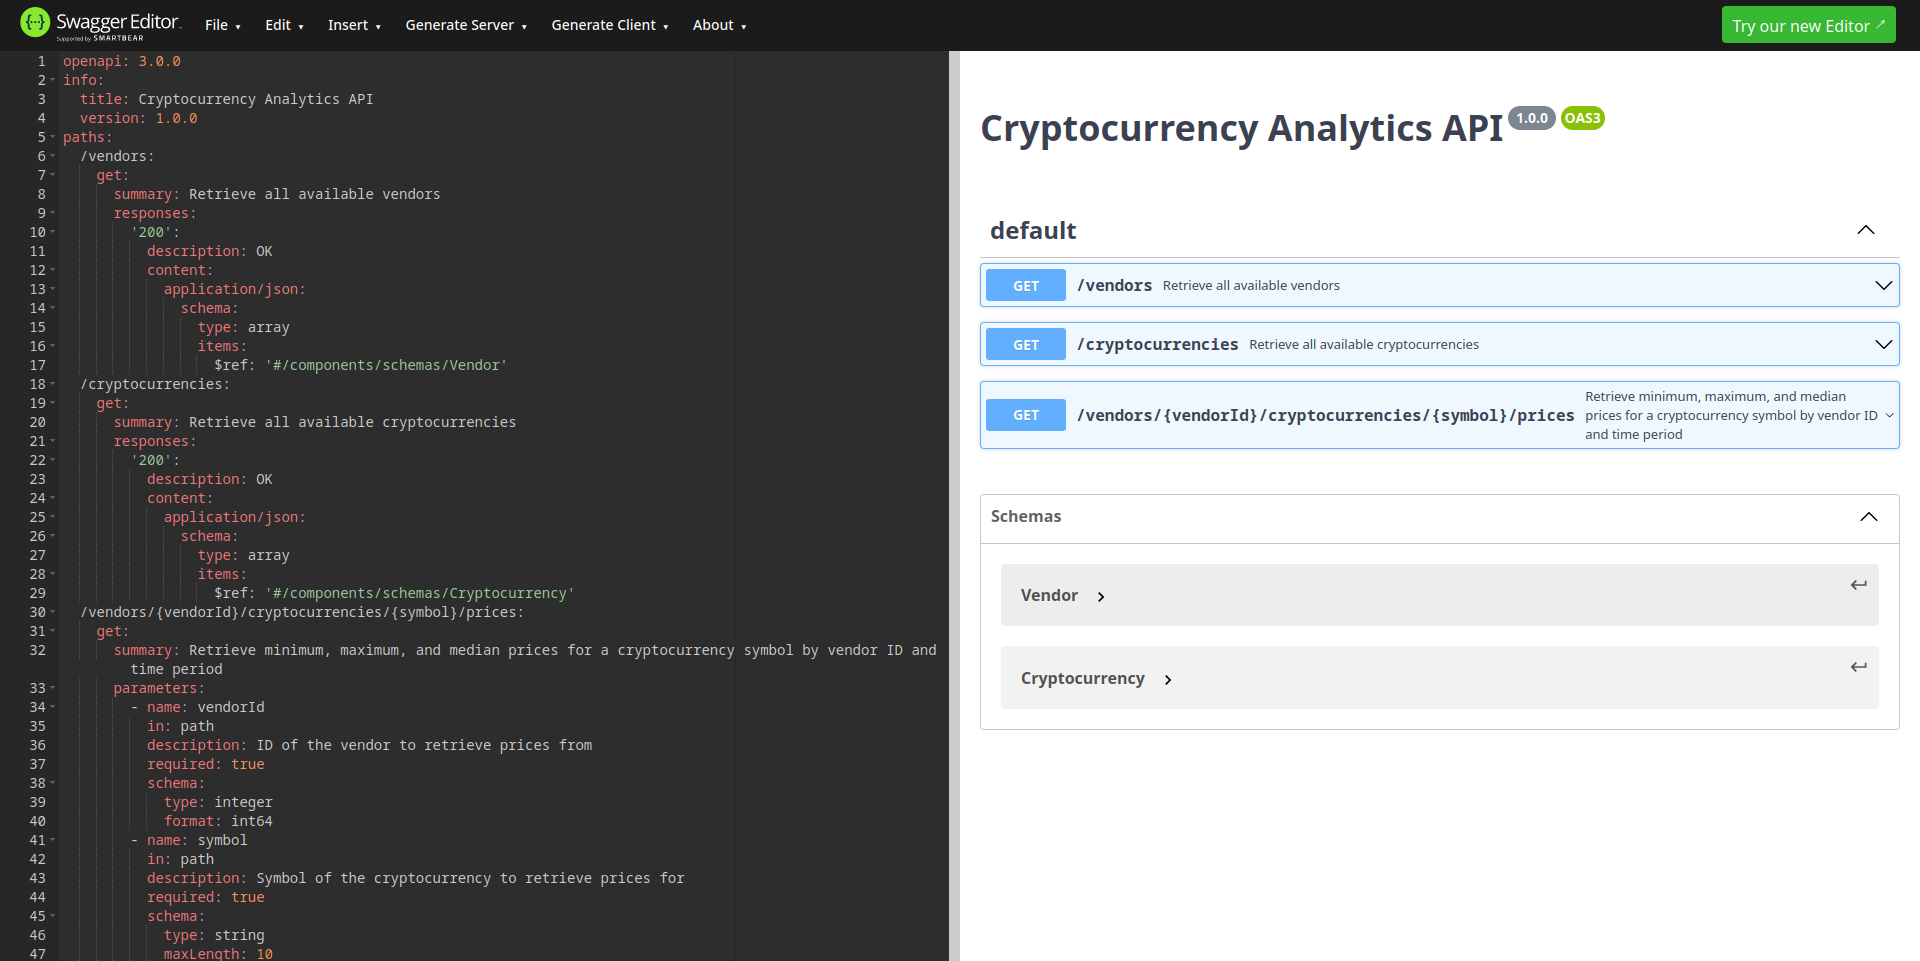
\includegraphics[width=1\linewidth]{swagerscreen.png}
    \caption{Изображение Swagger Editor с документацией к API приложения}
    \label{swager}
\end{figure}

OpenAPI документация помогает разработчикам легко создавать и поддерживать API,
а также упрощает процесс интеграции с другими приложениями. Она также
обеспечивает единый стандарт для описания API, что позволяет разработчикам легко
понимать и использовать API других приложений.

Приложение также может работать как автономное приложение, если
подключиться к Grafana и смотреть цены на криптовалюту используя
разработанный дашборд (см. Рис \ref{grafana}).
Grafana --- это инструмент для визуализации данных,
который позволяет отображать данные в режиме реального времени. Дашборд
позволяет отслеживать цены на криптовалюту в режиме реального времени и
анализировать изменения цен с помощью графиков и диаграмм.

Таким образом, в рамках разработки распределенной асинхронной системы
обработки real-time финансовых данных было уделено большое внимание
документированию API приложения. Использование OpenAPI позволило
легко создавать и поддерживать API, а также упрощал процесс интеграции с другими
приложениями. Итоговое приложение также может работать как автономное приложение,
если подключиться к Grafana и использовать разработанный дашборд для
отслеживания цен на криптовалюту в режиме реального времени.